\documentclass[12pt,a4paper]{article}
\usepackage[utf8]{vietnam}
\usepackage{amsmath,amssymb}
\usepackage{tabularx}
\usepackage{tikz}
\usetikzlibrary{calc,angles,quotes,arrows.meta}
\usepackage{xcolor}
\usepackage{enumitem}
\usepackage{fancyhdr}
\usepackage[top=1.2cm, bottom=1.2cm, left=1.5cm, right=1.5cm]{geometry}
\usepackage[dethi]{ex_test}
\SAOPTN{widthSA=2.6,heightSA=0.62}

\setlength{\headheight}{15pt}
\setlength{\parskip}{0pt}

% Dòng kẻ chấm mờ chuẩn viết tay
\newcommand{\dongke}[1]{%
  \begingroup%
  \setlength{\parskip}{0pt}%
  \baselineskip=18.5pt%
  \vspace{1.0mm}%
  \foreach \i in {1,...,#1}{%
    \noindent{\color{gray!60}\dotfill}\par%
  }%
  \vspace{0.6mm}%
  \endgroup%
}

\pagestyle{fancy}
\fancyhf{}
\rhead{\textit{Môn Toán 7 -- Đề số 3}}
\lhead{\textit{Bộ đề ôn tập Giữa học kì I}}
\cfoot{\thepage}

\begin{document}

% --- KHUNG TIÊU ĐỀ ĐỀ THI ---
\noindent
\begin{tabularx}{\linewidth}{X r}
\textbf{TRƯỜNG THCS: \dotfill} & \textbf{ĐỀ KIỂM TRA ĐỊNH KỲ GIỮA HỌC KỲ I} \\
\textbf{Họ và tên: \dotfill} & \textbf{NĂM HỌC 2026 -- 2027} \\
\textbf{Lớp: \dotfill \quad SBD: \dotfill} & \textbf{Môn: TOÁN 7} \\
& \textit{Thời gian làm bài: 90 phút (không kể thời gian phát đề)}
\end{tabularx}

\vspace{1.5mm}
\noindent
\begin{tabularx}{\linewidth}{|p{3.5cm}|X|}
\hline
\centering\textbf{Điểm số} & \centering\textbf{Lời nhận xét của thầy cô giáo} \tabularnewline
\rule{0pt}{1.6cm} & \\
\hline
\end{tabularx}

\vspace{2.5mm}
\begin{center}
\textbf{\large ĐỀ SỐ 3}
\end{center}

\noindent\textbf{\large PHẦN I. CÂU TRẮC NGHIỆM NHIỀU PHƯƠNG ÁN LỰA CHỌN (3,0 điểm)}

\textit{Thí sinh trả lời từ câu 1 đến câu 12. Mỗi câu hỏi chỉ chọn một phương án đúng nhất và ghi vào bảng đáp án.}

\vspace{1mm}
\begin{ex}
Số đối của số $\dfrac{1}{3}$ là:
\choice
{$3$}
{\True $-\dfrac{1}{3}$}
{$\dfrac{3}{5}$}
{$-0{,}2$}
\end{ex}

\begin{ex}
\immini{
Từ hình sau, góc $x'Oy'$ đối đỉnh với góc nào?
\choice
{\True $\widehat{xOy}$}
{$\widehat{y'Ox}$}
{$\widehat{x'Oy}$}
{$\widehat{xOy'}$}
}{
\begin{tikzpicture}[scale=0.9, line cap=round, line join=round]
  \coordinate (O) at (0,0);
  \draw[thick] (-2.6,0) node[above=2pt] {$x$} -- (2.6,0) node[below=2pt] {$x'$};
  \draw[thick] (-2.2,-1.54) node[above left=1pt] {$y$} -- (2.2,1.54) node[above right=1pt] {$y'$};
  \node[above=3pt] at (O) {$O$};
\end{tikzpicture}
}
\end{ex}

\begin{ex}
Cho bài toán $x + \dfrac{1}{2} = 5$, khi chuyển số hạng $\dfrac{1}{2}$ từ vế trái sang vế phải ta được:
\choice
{$x = 5 + \dfrac{1}{2}$}
{$x = -5 + \dfrac{1}{2}$}
{\True $x = 5 - \dfrac{1}{2}$}
{$x = -5 - \dfrac{1}{2}$}
\end{ex}

\begin{ex}
Tia $Ot$ nào trong các hình dưới đây là tia phân giác của góc $\widehat{xOy}$?
\begin{center}
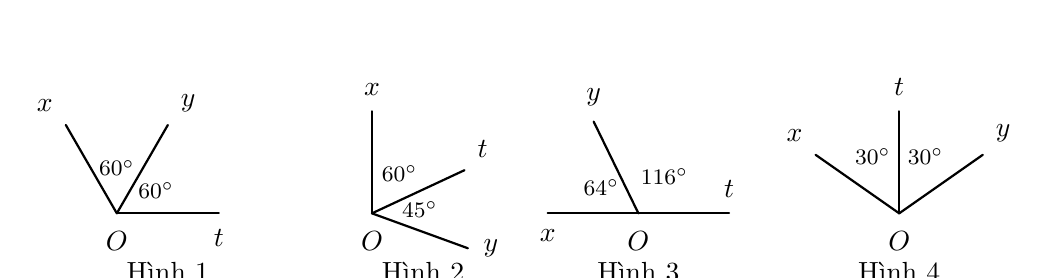
\begin{tikzpicture}[scale=0.72, line cap=round, line join=round, thick]
  % Hình 1
  \begin{scope}[shift={(0,0)}]
    \coordinate (O) at (0,0);
    \draw (O) -- (1.8,0) node[below=2pt] {$t$};
    \draw (O) -- (60:1.8) node[above right=1pt] {$y$};
    \draw (O) -- (120:1.8) node[above left=1pt] {$x$};
    \node[font=\footnotesize] at (30:0.8) {$60^\circ$};
    \node[font=\footnotesize] at (90:0.8) {$60^\circ$};
    \node[below=3pt] at (O) {$O$};
    \node[below=14pt] at (0.9,0) {Hình 1};
  \end{scope}
  % Hình 2
  \begin{scope}[shift={(4.5,0)}]
    \coordinate (O) at (0,0);
    \draw (O) -- (0,1.8) node[above=2pt] {$x$};
    \draw (O) -- (25:1.8) node[above right=1pt] {$t$};
    \draw (O) -- (-20:1.8) node[right=2pt] {$y$};
    \node[font=\footnotesize] at (55:0.85) {$60^\circ$};
    \node[font=\footnotesize] at (5:0.85) {$45^\circ$};
    \node[below=3pt] at (O) {$O$};
    \node[below=14pt] at (0.9,0) {Hình 2};
  \end{scope}
  % Hình 3
  \begin{scope}[shift={(9.2,0)}]
    \coordinate (O) at (0,0);
    \draw (-1.6,0) node[below=2pt] {$x$} -- (1.6,0) node[above=2pt] {$t$};
    \draw (O) -- (116:1.8) node[above=2pt] {$y$};
    \node[font=\footnotesize] at (55:0.8) {$116^\circ$};
    \node[font=\footnotesize] at (145:0.8) {$64^\circ$};
    \node[below=3pt] at (O) {$O$};
    \node[below=14pt] at (0,0) {Hình 3};
  \end{scope}
  % Hình 4
  \begin{scope}[shift={(13.8,0)}]
    \coordinate (O) at (0,0);
    \draw (O) -- (0,1.8) node[above=2pt] {$t$};
    \draw (O) -- (145:1.8) node[above left=1pt] {$x$};
    \draw (O) -- (35:1.8) node[above right=1pt] {$y$};
    \node[font=\footnotesize] at (115:1.1) {$30^\circ$};
    \node[font=\footnotesize] at (65:1.1) {$30^\circ$};
    \node[below=3pt] at (O) {$O$};
    \node[below=14pt] at (0,0) {Hình 4};
  \end{scope}
\end{tikzpicture}
\end{center}
\choice
{Hình 1}
{Hình 2}
{Hình 3}
{\True Hình 4}
\end{ex}

\begin{ex}
Kết quả của phép tính $7^{10} : 7$ viết dưới dạng lũy thừa là:
\choice
{\True $7^9$}
{$7^{11}$}
{$7^{10}$}
{$1^{10}$}
\end{ex}

\begin{ex}
Nếu một đường thẳng cắt hai đường thẳng song song thì hai góc so le trong:
\choice
{\True Bằng nhau}
{Phụ nhau}
{Kề nhau}
{Kề bù}
\end{ex}

\begin{ex}
Cho các số thập phân sau: $0{,}12222\dots$; $4{,}(5)$; $1{,}2184218$; $-11{,}2(312)$. Số thập phân hữu hạn là:
\choice
{\True $1{,}2184218$}
{$0{,}12222\dots$}
{$4{,}(5)$}
{$-11{,}2(312)$}
\end{ex}

\begin{ex}
Qua một điểm ở ngoài một đường thẳng, có bao nhiêu đường thẳng song song với đường thẳng đó?
\choice
{Không có}
{Có vô số}
{Có ít nhất một}
{\True Chỉ có một}
\end{ex}

\begin{ex}
Số hữu tỉ $x$ thỏa mãn $x^2 = 25$ là:
\choice
{$625$}
{$-5$}
{$5$}
{\True $5$ hoặc $-5$}
\end{ex}

\begin{ex}
Mô tả quy tắc chuyển vế qua đẳng thức $x - \dfrac{1}{2} = -\dfrac{5}{6}$ ta được:
\choice
{$x - \dfrac{5}{6} = \dfrac{1}{2}$}
{$x = \dfrac{5}{6} + \dfrac{1}{2}$}
{\True $x = -\dfrac{5}{6} + \dfrac{1}{2}$}
{$x = -\dfrac{5}{6} - \dfrac{1}{2}$}
\end{ex}

\begin{ex}
Cho 3 đường thẳng phân biệt $a, b, c$. Biết $a \perp b$ và $b \perp c$, khi đó:
\choice
{$a \perp c$}
{$b \parallel c$}
{$a \parallel b$}
{\True $a \parallel c$}
\end{ex}

\begin{ex}
Căn bậc hai số học của $64$ là:
\choice
{$32$}
{$8$ và $-8$}
{$-8$}
{\True $8$}
\end{ex}


\vspace{1mm}
\noindent\textbf{BẢNG TRẢ LỜI TRẮC NGHIỆM PHẦN I:}
\begin{center}
\begin{tabular}{|c|c|c|c|c|c|c|c|c|c|c|c|c|}
\hline
\textbf{Câu} & \textbf{1} & \textbf{2} & \textbf{3} & \textbf{4} & \textbf{5} & \textbf{6} & \textbf{7} & \textbf{8} & \textbf{9} & \textbf{10} & \textbf{11} & \textbf{12} \\
\hline
\textbf{Chọn} & \rule{0pt}{0.65cm} & & & & & & & & & & & \\
\hline
\end{tabular}
\end{center}
\vspace{2mm}

\setcounter{ex}{0}
\noindent\textbf{\large PHẦN II. CÂU TRẮC NGHIỆM ĐÚNG SAI (2,0 điểm)}

\textit{Thí sinh trả lời câu 1 và câu 2. Trong mỗi ý a), b), c), d) ở mỗi câu, thí sinh chọn đúng hoặc sai.}

\vspace{1mm}
\begin{ex}
\immini{
Cho $\widehat{xOy} = 70^\circ$. Trên tia $Ox$ lấy điểm $A$. Kẻ tia $Az$ sao cho $\widehat{xAz} = 70^\circ$. Trên tia $Az$ lấy điểm $B$, kẻ tia $Bt$ cắt $Oy$ tại $C$ sao cho $\widehat{CBA} = 110^\circ$. Xét tính đúng sai của các mệnh đề sau:
\choiceTF
{\True $\widehat{ABC}$ và $\widehat{CBz}$ là hai góc kề bù}
{\True $\widehat{CBz} = 70^\circ$}
{\True $Oy$ song song với $Az$}
{$\widehat{BCO} = 110^\circ$}
}{
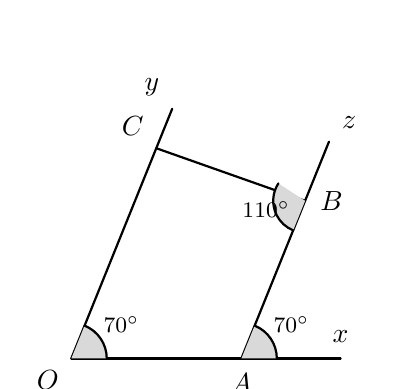
\begin{tikzpicture}[scale=0.9, line cap=round, line join=round]
  \coordinate (O) at (0,0);
  \coordinate (A) at (2.4,0);
  \coordinate (B) at ($(A)+(68:2.4)$);
  \coordinate (C) at ($(O)+(68:3.2)$);
  \draw[thick] (O) -- (3.8,0) node[above=2pt] {$x$};
  \draw[thick] (O) -- ($(O)+(68:3.8)$) node[above left=1pt] {$y$};
  \draw[thick] (A) -- ($(A)+(68:3.3)$) node[above right=1pt] {$z$};
  \draw[thick] (C) -- (B);
  \fill[gray!30] (O) -- (0.5,0) arc (0:68:0.5) -- cycle;
  \draw[thick] (0.5,0) arc (0:68:0.5);
  \node[font=\footnotesize] at (34:0.85) {$70^\circ$};
  \fill[gray!30] (A) -- ++(0:0.5) arc (0:68:0.5) -- cycle;
  \draw[thick] (A) ++(0:0.5) arc (0:68:0.5);
  \node[font=\footnotesize] at ($(A)+(34:0.85)$) {$70^\circ$};
  \fill[gray!30] (B) -- ++(147:0.45) arc (147:248:0.45) -- cycle;
  \draw[thick] (B) ++(147:0.45) arc (147:248:0.45);
  \node[font=\footnotesize] at ($(B)+(-0.55,-0.12)$) {$110^\circ$};
  \node[below left=1pt] at (O) {$O$};
  \node[below=2pt] at (A) {$A$};
  \node[right=2pt] at (B) {$B$};
  \node[above left=1pt] at (C) {$C$};
\end{tikzpicture}
}
\end{ex}

\begin{ex}
Cho biểu thức $M = \left(-\dfrac{1}{2}\right)^3 \cdot \dfrac{8}{3} + \left|-\dfrac{3}{4}\right|$. Xét tính đúng sai của các mệnh đề sau:
\choiceTF
{\True Giá trị của lũy thừa $\left(-\dfrac{1}{2}\right)^3$ bằng $-\dfrac{1}{8}$}
{Giá trị tuyệt đối $\left|-\dfrac{3}{4}\right|$ bằng $-\dfrac{3}{4}$}
{Giá trị của biểu thức $M$ bằng $-\dfrac{1}{4}$}
{Giá trị $M$ tìm được là một số hữu tỉ âm}
\end{ex}


\noindent\textbf{BẢNG TRẢ LỜI PHẦN II:}
\begin{center}
\begin{tabular}{|c|c|c|c|c||c|c|c|c|c|}
\hline
\textbf{Câu 1} & \textbf{a)} & \textbf{b)} & \textbf{c)} & \textbf{d)} & \textbf{Câu 2} & \textbf{a)} & \textbf{b)} & \textbf{c)} & \textbf{d)} \\
\hline
\textbf{Đ/S} & \rule{0pt}{0.6cm} & & & & \textbf{Đ/S} & & & & \\
\hline
\end{tabular}
\end{center}
\vspace{2mm}

\setcounter{ex}{0}
\noindent\textbf{\large PHẦN III. CÂU HỎI TRẢ LỜI NGẮN (1,0 điểm)}

\textit{Thí sinh trả lời câu 1 và câu 2. Điền kết quả vào ô trống.}

\vspace{1mm}
\begin{ex}
Tìm số hữu tỉ $x$, biết: $\left(x - \dfrac{1}{3}\right)^2 = \dfrac{4}{9}$. \shortans{$x \in \left\{1; -\dfrac{1}{3}\right\}$}
\end{ex}

\begin{ex}
Cho hai đường thẳng $xx'$ và $yy'$ cắt nhau tại điểm $O$. Biết $\widehat{xOy} = 60^\circ$. Tính số đo góc đối đỉnh $\widehat{x'Oy'}$ và góc kề bù $\widehat{x'Oy}$ với góc $\widehat{xOy}$. \shortans{$\widehat{x'Oy'} = 60^\circ; \widehat{x'Oy} = 120^\circ$}
\end{ex}


\setcounter{ex}{0}
\noindent\textbf{\large PHẦN IV. TỰ LUẬN (4,0 điểm)}

\textit{Thí sinh trình bày chi tiết lời giải vào giấy làm bài.}

\vspace{1mm}
\begin{ex}
Thực hiện phép tính:
\begin{enumerate}[label=\textbf{\alph*)}, leftmargin=0.8cm, itemsep=1pt]
\item $(-0{,}25) \cdot 40 + 3 + 2026^0$
\item $\dfrac{1}{7} \cdot \dfrac{-3}{8} + \dfrac{-13}{8} \cdot \dfrac{1}{7}$
\item $\left[ \left(\dfrac{2}{3} - \dfrac{7}{6}\right)^2 + (-2)^3 \cdot 3 \right] : 4\dfrac{3}{4} - 1$
\end{enumerate}
\end{ex}
\vspace{1.5mm}

\begin{ex}
Tìm $x$ biết:
\begin{enumerate}[label=\textbf{\alph*)}, leftmargin=0.8cm, itemsep=1pt]
\item $x + 4{,}5 = 9{,}5$
\item $\dfrac{2}{5} \cdot x - \dfrac{1}{2} = \dfrac{3}{8}$
\item $|3x - 1| + \dfrac{1}{3} = \dfrac{1}{2}$
\end{enumerate}
\end{ex}
\vspace{1.5mm}

\begin{ex}
Hai người thợ cùng làm một công việc. Nếu làm riêng thì người thứ nhất phải mất 3 giờ, người thứ hai phải mất 5 giờ mới hoàn thành công việc. Hỏi nếu làm chung trong 45 phút thì hai người làm được mấy phần công việc?
\end{ex}
\vspace{1.5mm}


\begin{center}
\rule{4cm}{0.4pt}\\
\textit{--- HẾT ---}
\end{center}
\end{document}
